\documentclass[a4paper]{report}
\usepackage[sorting=none]{biblatex}
\addbibresource{safe-devicelocatorui.bib}
\usepackage[T1]{fontenc}
\usepackage[utf8]{inputenc}
\usepackage[italian]{babel}
\usepackage{csquotes}
\usepackage{enumitem}
\usepackage{menukeys}
\begin{document}


\makeatletter

\newcommand\setnewpathsep[1]
{%
    \tw@declare@style@simple*{paths}{%
       {\ttfamily\CurrentMenuElement}%
    }[%
       #1%
    ]{blacknwhite}
}

\author{Lorenzo Tanganelli \and Luca Patarca \and Nico Trionfetti}
\title{Safe-Device Locator UI}
\maketitle

\newpage
\tableofcontents

\newpage

\addcontentsline{toc}{section}{Introduzione}
\section*{{Introduzione}}
Il progetto di ricerca industriale \citetitle{SAFE}\cite{SAFE} ha come obbiettivo la realizzazione di sistemi di arredo innovativi capaci di trasformarsi in sistemi inteligenti di protezione passiva delle persone in caso di crollo dell'edificio causato da un terremoto.

Questi sistemi di arredo smart saranno dotati di sensoristica "salva-vita" capace di pre-allertare in caso di terremoto, di rilevare e localizzare la presenza di vita dopo un crollo, di monitorare le condizioni ambientali sotto le macerie e di elaborare e trasmettere informazioni utili a chi deve portare soccorso.

Il ciclo di vita dei sensori si divide in tre scenari operativi:
\begin{enumerate}[label=\roman{*}., ref=(\roman{*})]
    \item \textbf{Tempo di pace:} monitoraggio per il pre-allertamento (es. misure accellerometriche)
    \item \textbf{Durante l'evento:} invio dei dati per il rilevamento dei danni (es. misure accellerometriche, inclinometriche e di spostamento) e attivazione di logiche di intervento in seguito al riconoscimento dell'evento.
    \item \textbf{Dopo l'evento:} invio dei dati per la localizzazione delle vittime e monitoraggio ambientale al fine di guidare gli operatori nel triage di soccorso.
    \end{enumerate}

L'invio di dati tra i sensori ed il mondo esterno avviene utilizzando la tecnologia LoRa.\newline
LoRa consente trasmissioni a lungo raggio e a basso consumo energetico arrivando oltre 10 km nelle zone rurali e 3–5 km in zone fortemente urbanizzate.\cite{s18030772}

Facendo riferimento al modello ISO/OSI la tecnologia è presente in due strati: 
\begin{itemize}
    \item \textbf{LoRa: } Il livello fisico LoRa è proprietario della Semtech e non se ne conoscono i dettagli implementativi.
    LoRa utilizza una modulazione a spettro espanso proprietaria, derivata della modulazione Chirp Spread Spectrum (CSS). Inoltre utilizza la codifica Forward Error Correction (FEC) come meccanismo di rilevazione e successiva correzione degli errori contro le interferenze. 
    \item \textbf{LoRaWAN: } LoRaWAN è un protocollo del livello Media Access Control (MAC) che lavora a livello di rete per la gestione delle comunicazioni tra gateway Low Power Wide Area Network (LPWAN) e dispositivi end-node come protocollo di routing.
    \end{itemize} 
Lo scenario operativo post evento si divide in tre attività:
\begin{enumerate}[label=\roman{*}., ref=(\roman{*})]
    \item \textbf{Campionatura:} mediante l'utilizzo di un drone dotato di tecnologia che supporta il protocollo LoRaWAN viene campionata l'area coperta dalle macerie. Durante la fase di volo vengono memorizzati i dati ricevuti dai sensori e la potenza del segnale.
    \item \textbf{Analisi dati:} sfruttando opportuni algoritmi di localizzazione vengono analizzati i dati memorizzati dal drone così da determinare dei centroidi in cui si suppone si trovi il disperso. 
    \item \textbf{Guidare soccorittori:} i soccorittori, dotati di opportuni tablet, visualizzerano una mappa con la heatmap e i centroidi risultanti dall'attività di analisi dati, così da potersi orientare per individuare i dispersi.
    \end{enumerate}

Il nostro progetto, all'interno di S.A.F.E.,  ha l'obbiettivo di creare un applicativo per tablet linux e android utile nell'ultima attività post evento.\newline 
Trovandosi in uno stato d'emergenza, l'applicazione punta ad avere un interfaccia grafica semplice e funzionale così da agevolare il lavoro degli operatori. Inoltre, dovrà essere in grado di funzionare senza connessione internet in quanto il terremoto potrebbe causare l'interruzione delle comunicazioni.

\addcontentsline{toc}{section}{Processo di sviluppo}
\section*{{Processo di sviluppo}}

\addcontentsline{toc}{subsection}{Prima iterazione}
\subsection*{{Prima iterazione}}

\addcontentsline{toc}{subsubsection}{Requisiti}
\subsubsection*{{Requisiti}}

Durante l'attività di analisi sono emersi i seguenti requisiti:
\begin{itemize}
    \item \textbf{Visualizzazione di una mappa}\newline Il soccorritore necessitta di una mappa sempre visibile del luogo in quanto potrebbe non conoscere la zona da soccorrere.
    \item \textbf{Rendering di dati vettoriali come heatmap}\newline La posizione del sensore individuata nella fase d'analisi dati potrebbe non essere corretta, quindi si prevede la possibilita di far visualizzare la heatmap degli RSSI all'operatore così da poter fare ulteriori supposizioni in base alle condizioni delle macerie e velocizzare il recupero del disperso.
    \item \textbf{Rendering di marker sulla base delle posizioni dei sensori}\newline Si necessita l'utilizzo di marker per visualizzare probabile la posizione del sensore.
    \item \textbf{Rendering di dati vettoriali come centroidi}\newline Si prevede la possibilità  di visualizzare poligoni con i marker come centroidi così da delimitare l'aria di ricerca.
    \item \textbf{Geolocalizzazione del dispositivo}\newline Le macerie degli edifici potrebbero aver ricoperto le strade e individuare la posizione GPS del dispositivo sopra la mappa può essere di supporto all'operatore per orientarsi.
    \item \textbf{Visualizzazione delle informazioni inviate dai sensori}\newline Conoscere lo stato di salute dei dispersi è fondamentale per i soccorittori, così da poter decidere a chi dare la precedenza durante il salvataggio.
    \item \textbf{Mantenimento dello stato nel caso in cui venga terminata l'applicazione}\newline Si prevede che l'applicativo mantenga il suo stato in caso di chiusura e successivo riavvio. Per esempio, se il dispositivo si dovesse scaricare, al riavvio l'applicazione dovrà trovarsi allo stato precedente lo spegnimento, così da minimizzare i tempi di attesa.
    \item \textbf{Funzionamento senza comunicazione internet}\newline Il terremoto potrebbe causare l'interruzione delle comunicazioni, per questo motivo si prevede che l'applicazioni non necessiti di internet per funzionare.
    \end{itemize} 
In questa iterazione abbiamo scelto di sviluppare questi requisiti:
\begin{itemize}
    \item Visualizzazione di mappe.
    \item Rendering di dati vettoriali come heatmap.
    \item Rendering di marker sulla base delle posizioni dei sensori.
    \item Visualizzazione delle informazioni inviate dai sensori.
    \item Funzionamento senza comunicazione internet.
    \end{itemize} 

\addcontentsline{toc}{subsubsection}{Progettazione e Implementazione}
\subsubsection*{{Progettazione e Implementazione}}
Terminata la prima attività di progettazione si é scelto di utilizzare il framework \citetitle{Flutter}\cite{Flutter} basato su \citetitle{Dart}\cite{Dart} per lo sviluppo del frontend, così da creare un applicazione nativa compilata sia per mobile che per desktop. Flutter utilizza i widget come elemento principale che consentono di risparmiare tempo nello sviluppo di elementi dell'interfaccia utente di base per ogni schermo e risoluzione. Flutter ha il proprio toolkit widget, ma tutti i componenti vengono renderizzati in modo nativo. Ciò conferisce alle app un aspetto nativo e migliora le prestazioni. Flutter è fondamentalmente un wrapper attorno a un'app che utilizza uno speciale metodo di comunicazione chiamato Platform Channels per connettere i dati alle lingue native. È facile da usare e consente agli sviluppatori di accedere all'hardware in quando dispone di librerie che consentono di collegarsi al chip GPS, fotocamera e microfono\cite*{FlutterMedium}.

Per visualizzare la mappa abbiamo deciso di appoggiarci all'implementazione Dart di Leaflet per Flutter denominata \citetitle{FlutterMap}\cite{FlutterMap}; Leaflet è la principale libreria JavaScript open source per mappe interattive ottimizzate per dispositivi mobili. Il pacchetto Flutter\_Map rende disponibili una serie di implementazioni della classe \textit{LayerOptions}, come per esempio \textit{CircleLayerOptions, MarkerLayerOptions, PolygonLayerOptions} e \textit{TileLayerOptions}, i quali permettono di fare il rendering della mappa e di aggiungerci informazioni. 
Purtoppo Flutter\_Map non dispone di un implementazione di LayerOptions per fare il rendering di una heatmap da aggiungere come layer alla mappa. Per questo motivo è stato deciso di adattare la classe CircleLayerOptions così da creare manualmente l'heatmap.

Invece, per lo state management, si è scelto di utilizzare il pacchetto \citetitle*{Provider}\cite{Provider} così da condividere i dati più facilmente nel widget tree. 
 
Per la generazione di mappe da utilizzare offline si è scelto di creare un eseguibile in \citetitle{Rust}\cite{Rust}. Rust è un linguaggio di programmazione multi-paradigma incentrato sulla sicurezza e sulle prestazioni, velocità ed efficienza. Rust risolve i problemi associati a C / C ++ come la garbage collection e la sicurezza\cite*{RustArticle}.


L'eseguibile in questione prende delle coordinaete geografiche in input, scarica i tiles in formato \textit{.png} e li organizza in cartelle nella seguente maniera:
\begin{center}
    {\setnewpathsep{/} \directory{./tiles/\{z\}/\{x\}/\{y\}/*.png}}
\end{center}
dove \{z\} indica lo zoom dell'immagine, mentre \{x\} e \{y\} indicano rispettivamente latitudine e longitudine.
Una volta terminato il processo di download la directory generata viene compressa nel file \textit{tiles.zip}
Si è deciso di scaricare le immagini da zoom 15 (scala 1:15 mila) a zoom 22 (scala 1:125) in un raggio di 5km dal punto centrale. Questa scelta è motivata dal fatto che vogliamo dare una visione generale di un quartiere o di un paese fino ad arrivare ad avere una visione dettagliata di singoli edifici.
%TODO Inserire informazioni riguardati i tiles!! formule utilizzate e aspetti tecnici + citazioni
Per scaricare la mappa da rendere disponibili offline ci appoggiamo a \citetitle{Thunderforest}\cite{Thunderforest}: un fornitore di tiles renderizzati dai dati di \citetitle{OpenStreetMap}\cite{OpenStreetMap}.

\addcontentsline{toc}{subsubsection}{Validazione e rilascio}
\subsubsection*{{Validazione e rilascio}}
Terminata l'attività di sviluppo del prototipo abbiamo soddisfatto quasi tutti i requisiti che ci eravamo prefissati per questa iterazione. Come si può notare dalla Figura \ref{marker_flutter} il prototipo visualizza una mappa con dei marker che cambiano il proprio aspetto in base allo stato del sensore: verde se è stato verificato, rosso altrimenti. Sulla sinistra si può notare la lista dei sensori con i relativi dati, in caso di tap sulla card del sensore la mappa sposta la visuale sopra le coordinaete del sensore selezionato. 
\begin{figure}[tbp]
    \centering
    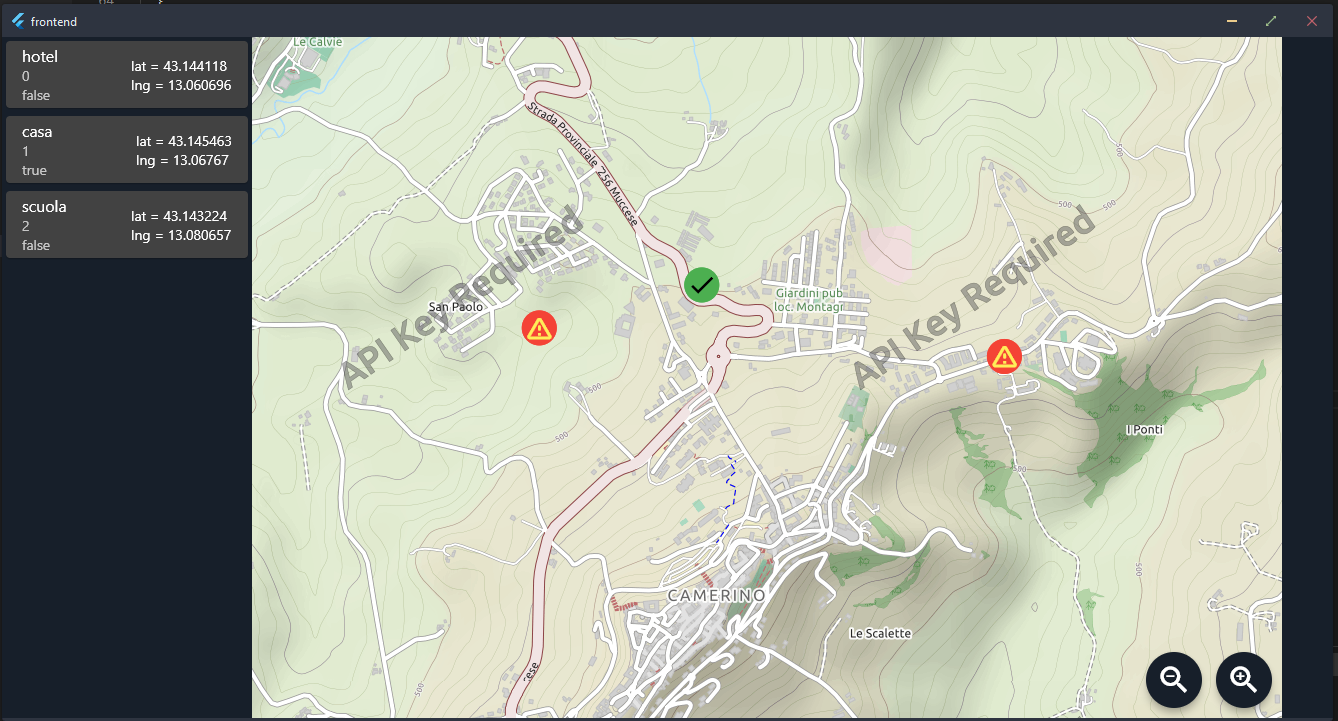
\includegraphics[width=\textwidth]{figure/marker_flutter.png}
    \caption{Marker Flutter}
    \label{marker_flutter}
\end{figure}

L'unico requisito che non è stato soddisfatto a pieno è stato quello di disegnare la heatmap, in quanto necessitavamo di visualizzare una mappa di calore che, in base alla scala della mappa, si ridisegnasse mettendo in relazione la distanza dei punti e l'RSSI rilevato (\textit{Received Signal Strength Indication}).

Come si può notare nella Figura~\ref{heatmap_flutter}, abbiamo disegnato dei punti che tenevano conto dell'RSSI ma non siamo stati in grado di tenere in considerazione la densità dei punti. Questo ci portava a visualizzare una heatmap che, se avevamo tanti punti vicino ma con intensità molto bassa venivano disegnati di verde, invece noi necessitavamo che in questa circostanza la zona interessata fosse colorata di rosso. 
\begin{figure}[tbp]
    \centering
    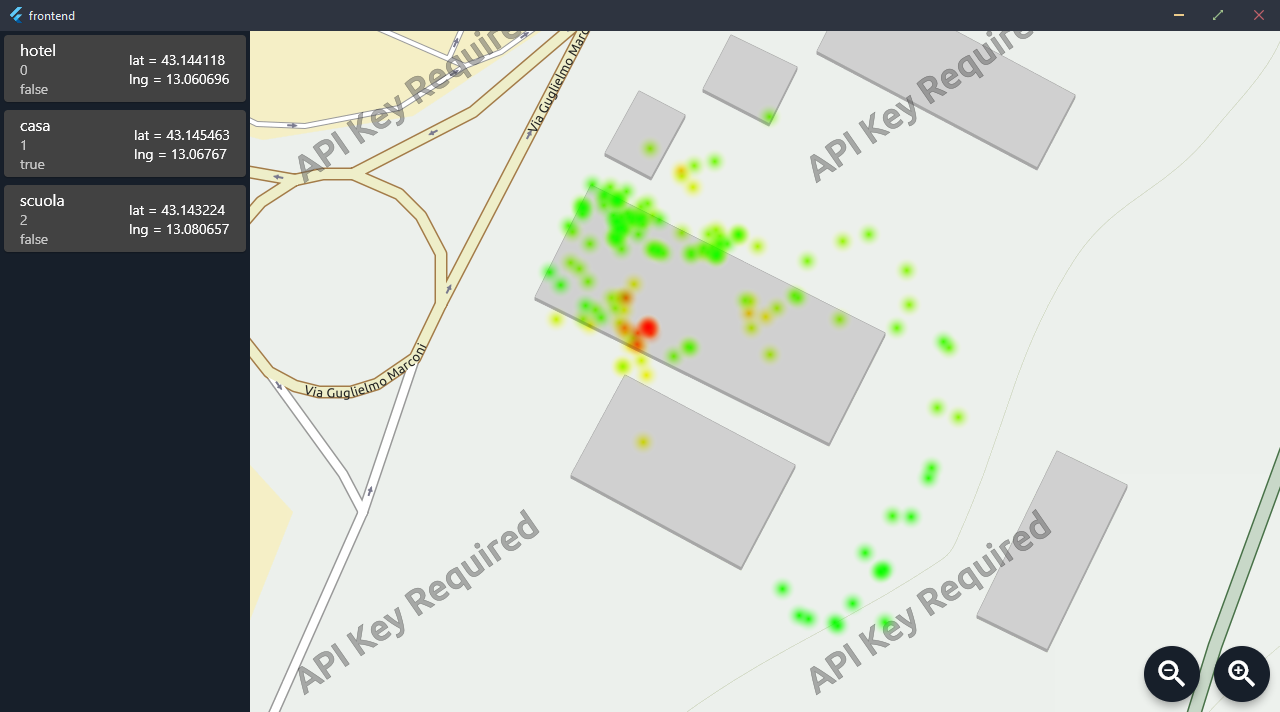
\includegraphics[width=.7\textwidth]{figure/heatmap_flutter_small.png}\hfill
    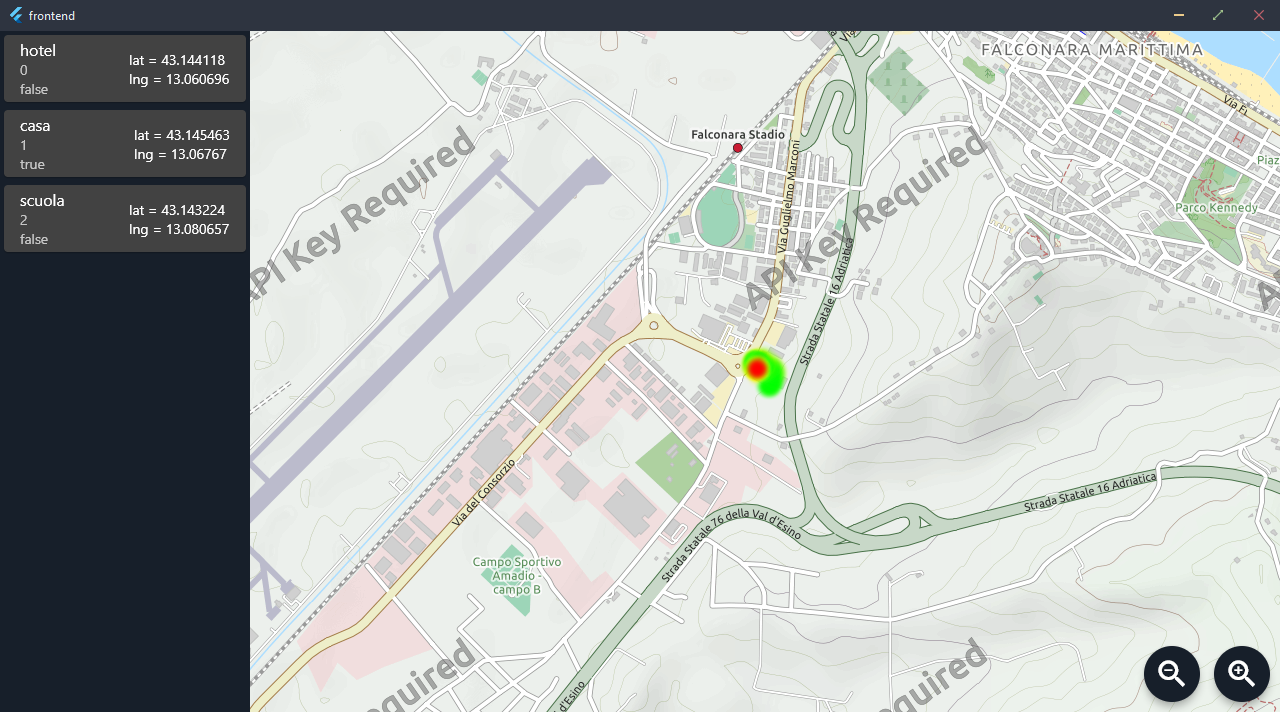
\includegraphics[width=.7\textwidth]{figure/heatmap_flutter_large.png}\hfill
    \caption{Heatmap Flutter}
    \label{heatmap_flutter}
\end{figure}

\addcontentsline{toc}{subsection}{Seconda iterazione}
\subsection*{{Seconda iterazione}}

Visti i feedback della precedente iterazione abbiamo deciso di mantenere i medesimi requisiti riguardanti il rendering della mappa ma di rivedere progettazione e implementazione cambiando tecnologie utilizzate. Questo cambiamento è motivato dal fatto che implementare un'heatmap che soddisfa il relativo requisito avrebbe richiesto più tempo che sviluppare un nuovo prototipo con una tecnologia differente, e per questo avremmo rischiato di non rispettare le scadenze. Della precendente iterazione abbiamo mantenuto l'eseguibile per rendere disponibili i tiles offline.

\addcontentsline{toc}{subsubsection}{Progettazione e Implementazione}
\subsubsection*{{Progettazione e Implementazione}}
In questa iterazione si è scelto di utilizzare il framework \citetitle*{IonicReact}\cite*{IonicReact}: versione \citetitle*{React}\cite*{React} di \citetitle*{Ionic}\cite*{Ionic}, per sviluppare il frontend. Abbiamo scelto Ionic React così da creare app per dispositivi mobili e desktop utilizzando \citetitle*{Capacitor}\cite*{Capacitor} e \citetitle*{Electron}\cite*{Electron}. 

Ionic è un framework di riferimento per lo sviluppo industriale. Le applicazioni aziendali sono, per loro natura, semplici e raramente funzionano con milioni di utenti: devono solo essere affidabili e intuitive. Ionic, quindi, risulta essere un framework affidabile che consente di ridurre i costi e la durata dello sviluppo pur offrendo un'esperienza utente eccellente e prestazioni stabili. \cite*{IonicReactArticle}

Ionic React utilizza standard web ed è compatibile con librerie web come \citetitle*{OpenLayers}\cite*{OpenLayers}: libreria che permette di visualizzare tiles, marker e dati vettoriali come heatmap e centroidi. 

Come mostrato in Figura \ref{IonicReact_2iterazione} si è scelto di mantenere la medesima struttura del primo prototipo per quanto riguarda la UI (\textit{User Interface}).
%TODO aggiungere informazioni sullo sviluppo 
\begin{figure}[tbp]
    \centering
    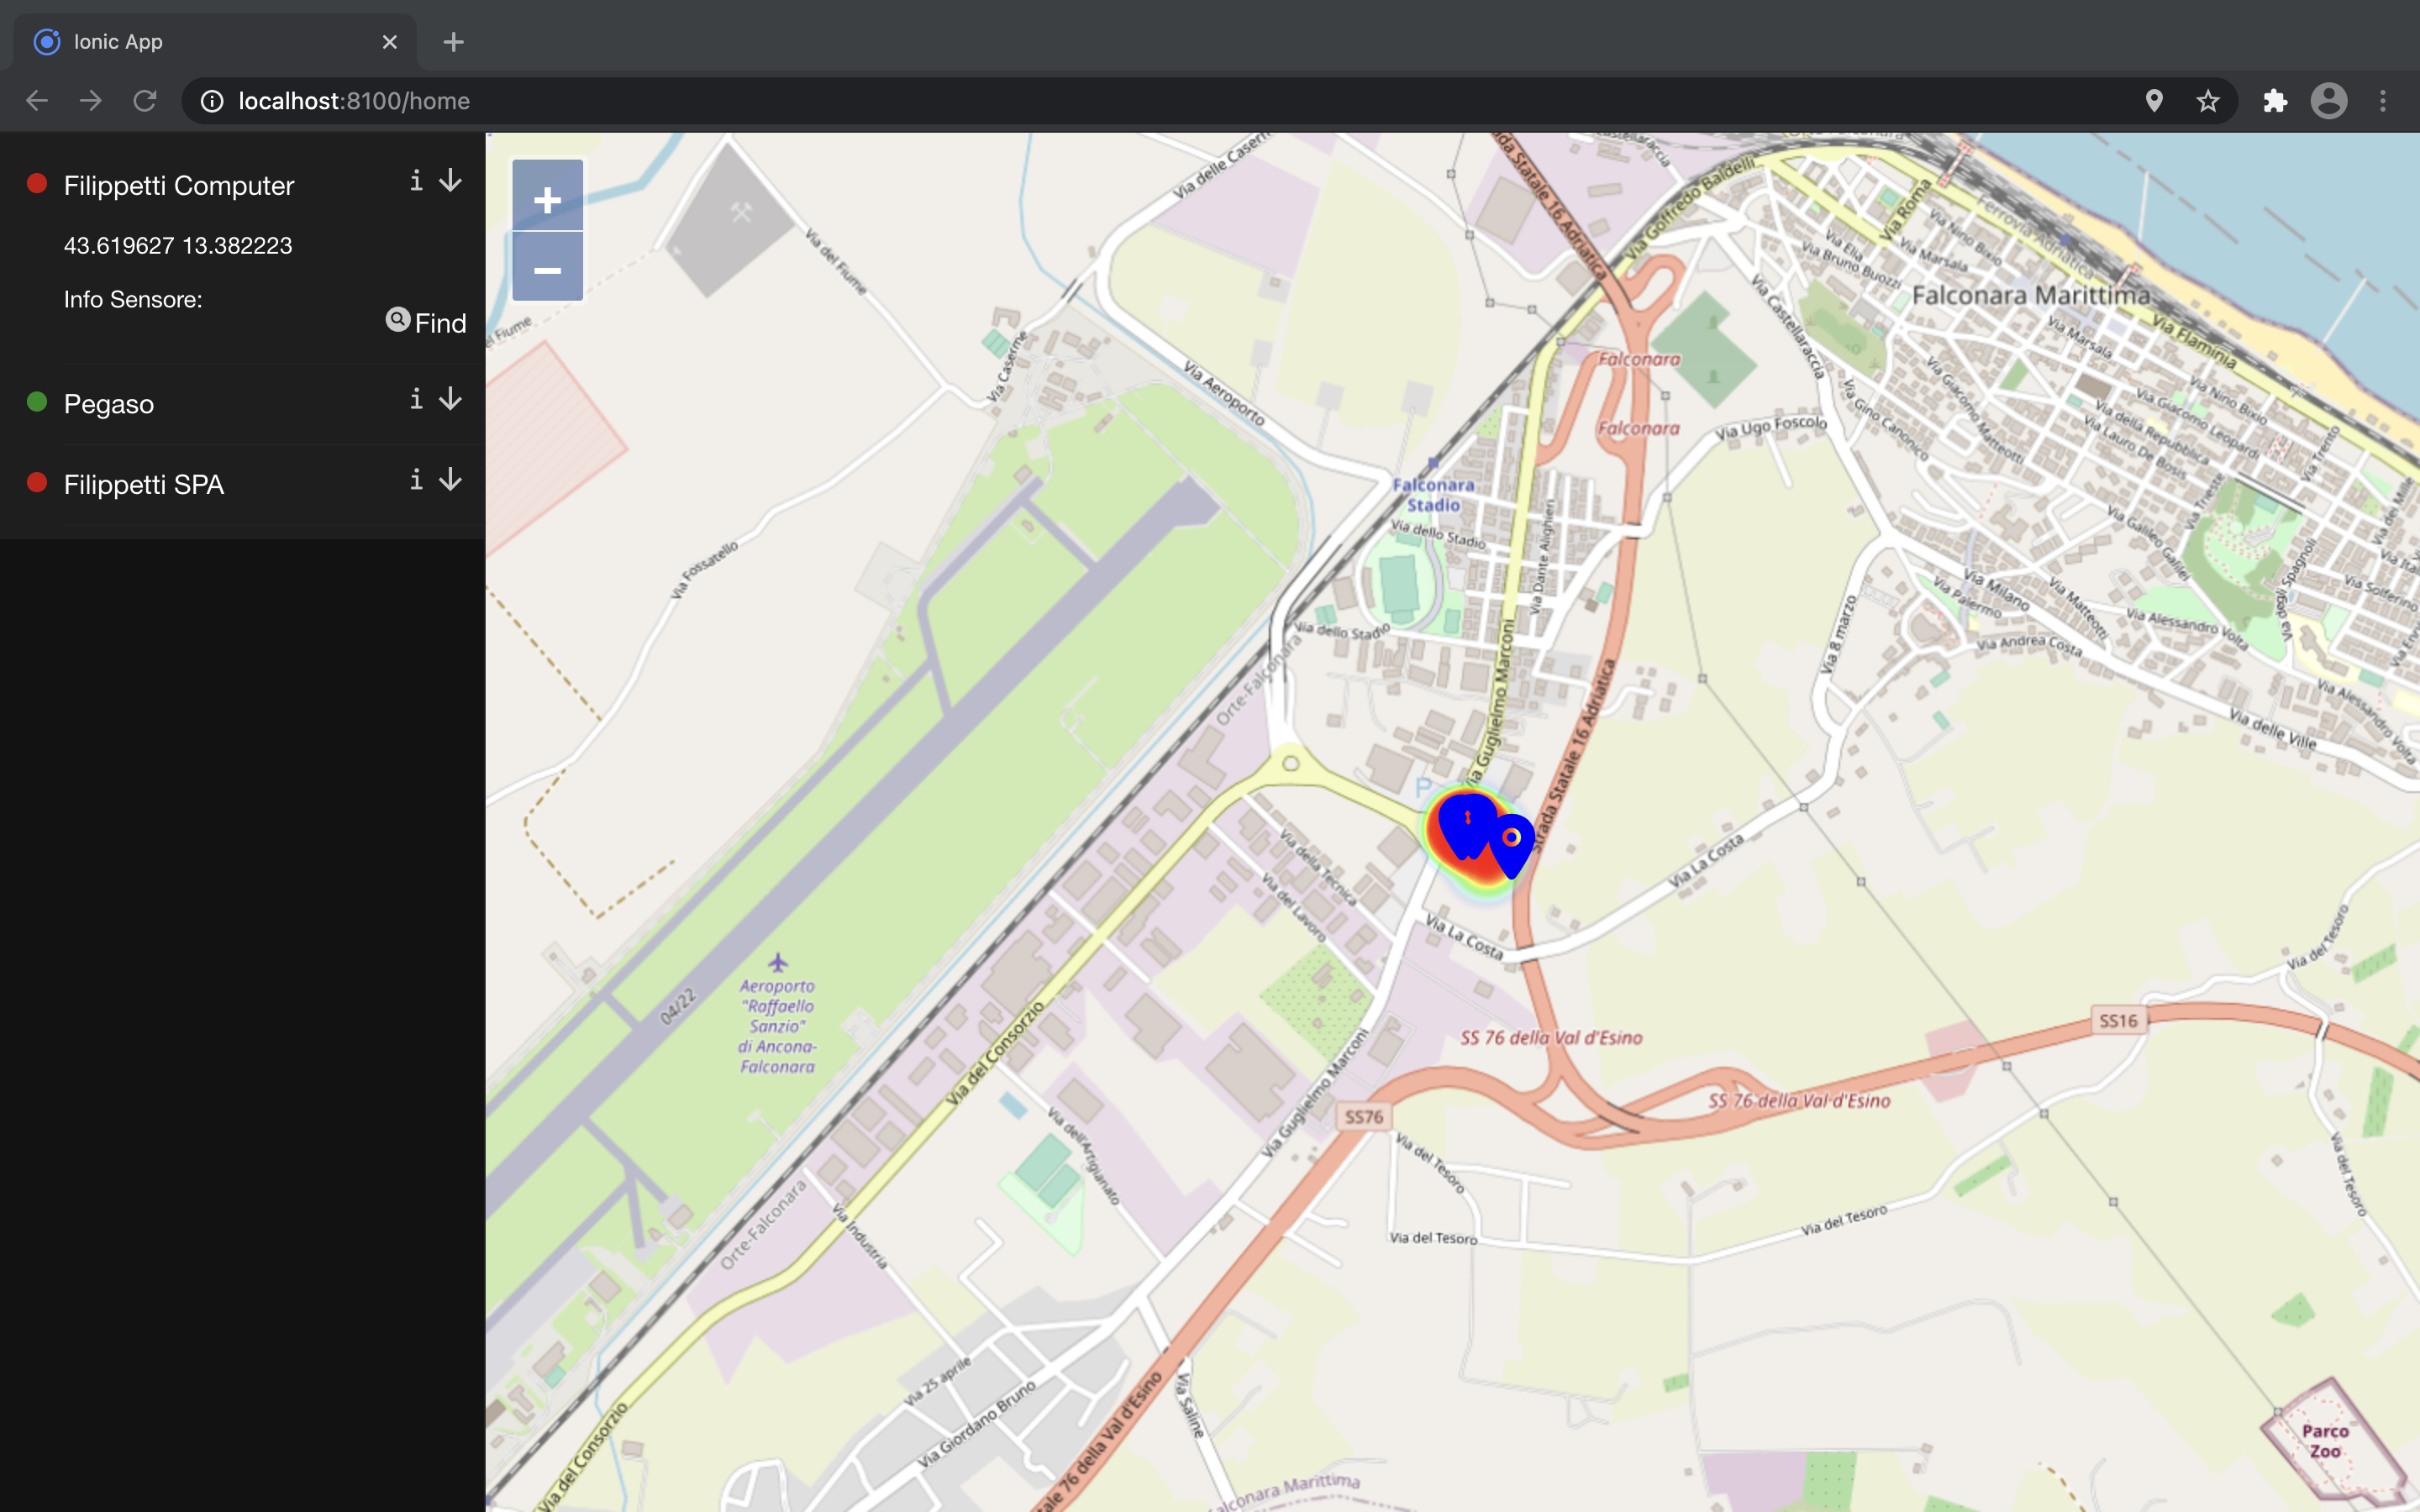
\includegraphics[width=.7\textwidth]{figure/ionicreact_2iterazione_large.png}\hfill
    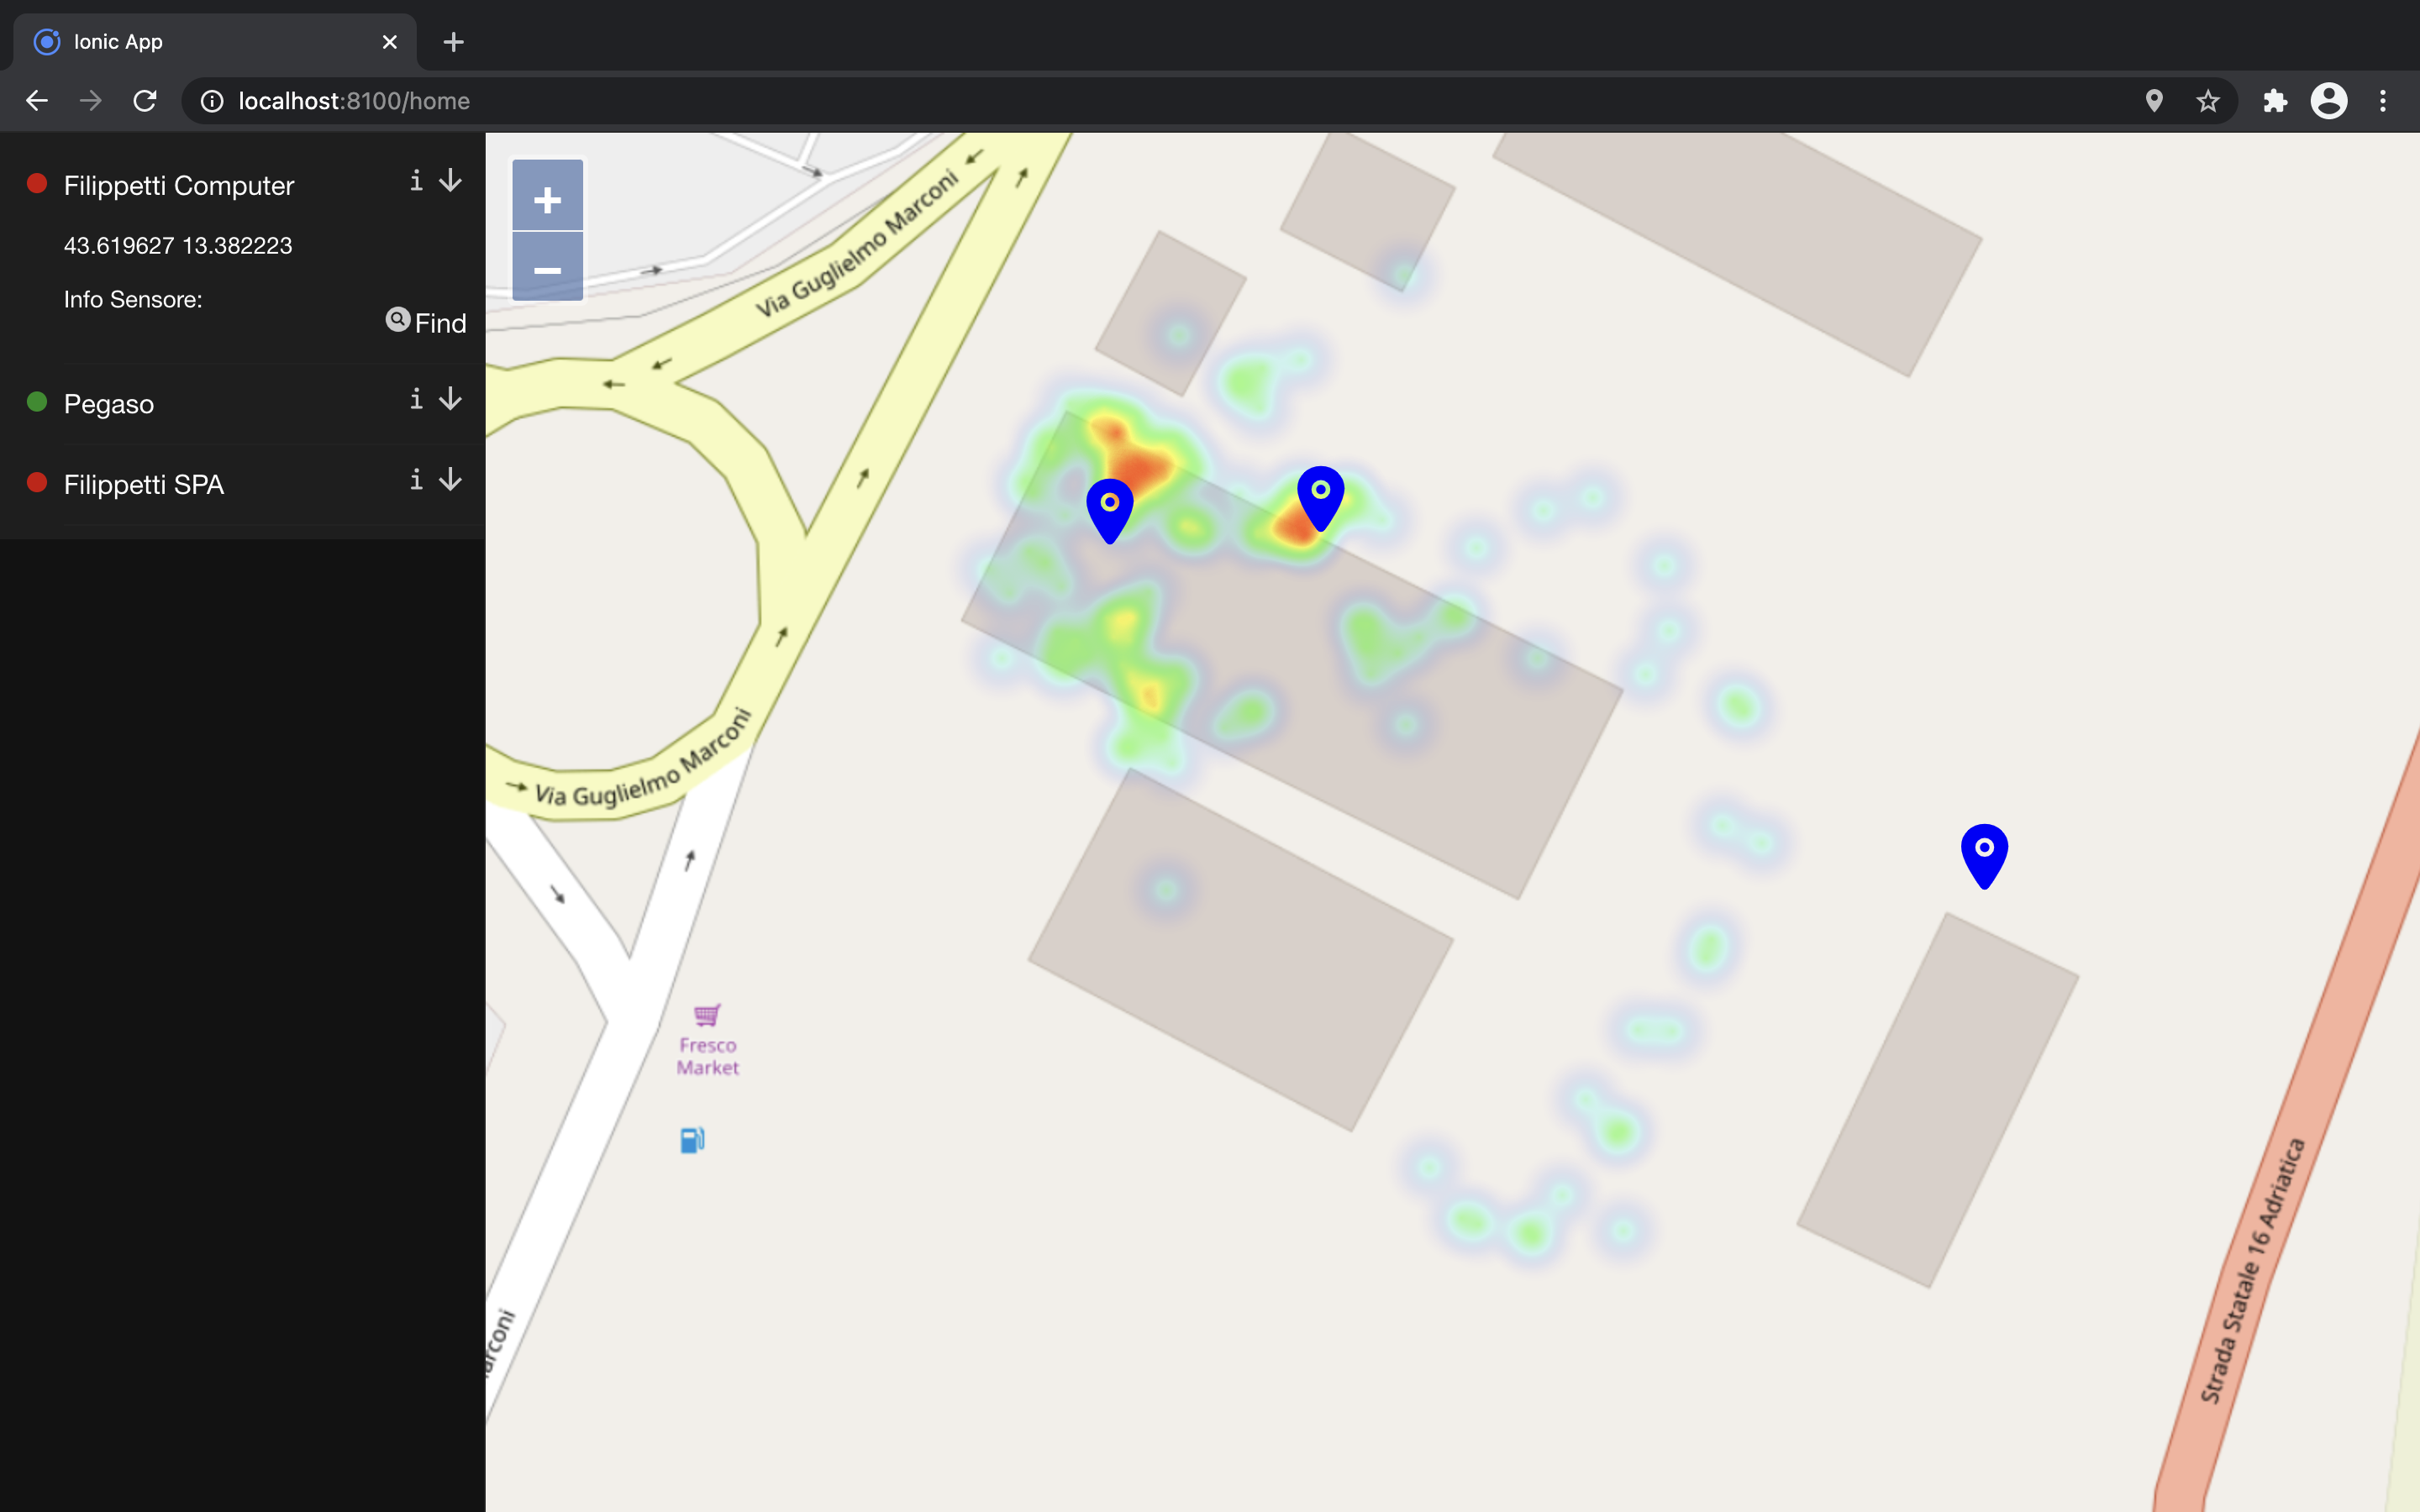
\includegraphics[width=.7\textwidth]{figure/ionicreact_2iterazione_small.png}\hfill

    \caption{IonicReact}
    \label{IonicReact_2iterazione}
\end{figure}

\addcontentsline{toc}{subsubsection}{Validazione e rilascio}
\subsubsection*{{Validazione e rilascio}}
Terminata l'attività di implementazione abbiamo soddisfatto tutti i requisiti che ci eravamo prefissati di sviluppare in questa iterazione. 

Si è notato che le informazioni aggiunte alla mappa, come marker e heatmap, possono essere elemento di disturbo nella situazione in cui l'operatote voglia visualizzare la mappa utilizzando una scala molto grande, per questo nelle prossime iterazioni si è scelto sviluppare un menu per selezionare quali layer mostrare.

\addcontentsline{toc}{subsection}{Terza iterazione}
\subsection*{{Terza iterazione}}

\addcontentsline{toc}{subsubsection}{Requisiti}
\subsubsection*{{Requisiti}}
Tra i requisiti individuati inizialmente abbiamo deciso di aggiungere, al prototipo validato nella precendente iterazione, le funzionalità riguardanti il requisito di geolocalizzazione del dispositivo.

Inoltre, si è deciso di implementare anche la funzionalità risultante dai feedback della seconda iterazione: un menù per selezionare quali layer mostrare sulla cartina.

\addcontentsline{toc}{subsubsection}{Progettazione e Implementazione}
\subsubsection*{{Progettazione e Implementazione}}
Come mostrato nella Figura \ref{IonicReact_3iterazione} sono stati aggiunti due bottoni sul lato destro dell'interfaccia. Il pulsante in alto a destra permette di visualizzare un menù all'interno di un popover contenente la lista dei layer disponibili e i relativi switch per abilitarne o meno la sovrampressione della mappa. Mentre, il pulsante nell'angolo inferiore destro, esegue le funzioni di geolocalizzazione e centra la visuale della mappa sulle coordinaete del dispositivo.
Per individuare la posizione geografica del dispositivo utilizziamo \citetitle*{cordova-plugin-geolocation}\cite*{cordova-plugin-geolocation} il quale sfrutta il sistema GPS o network signal: WiFi e GSM, per dedurre latitudine e longitudine.

\begin{figure}[tbp]
    \centering
    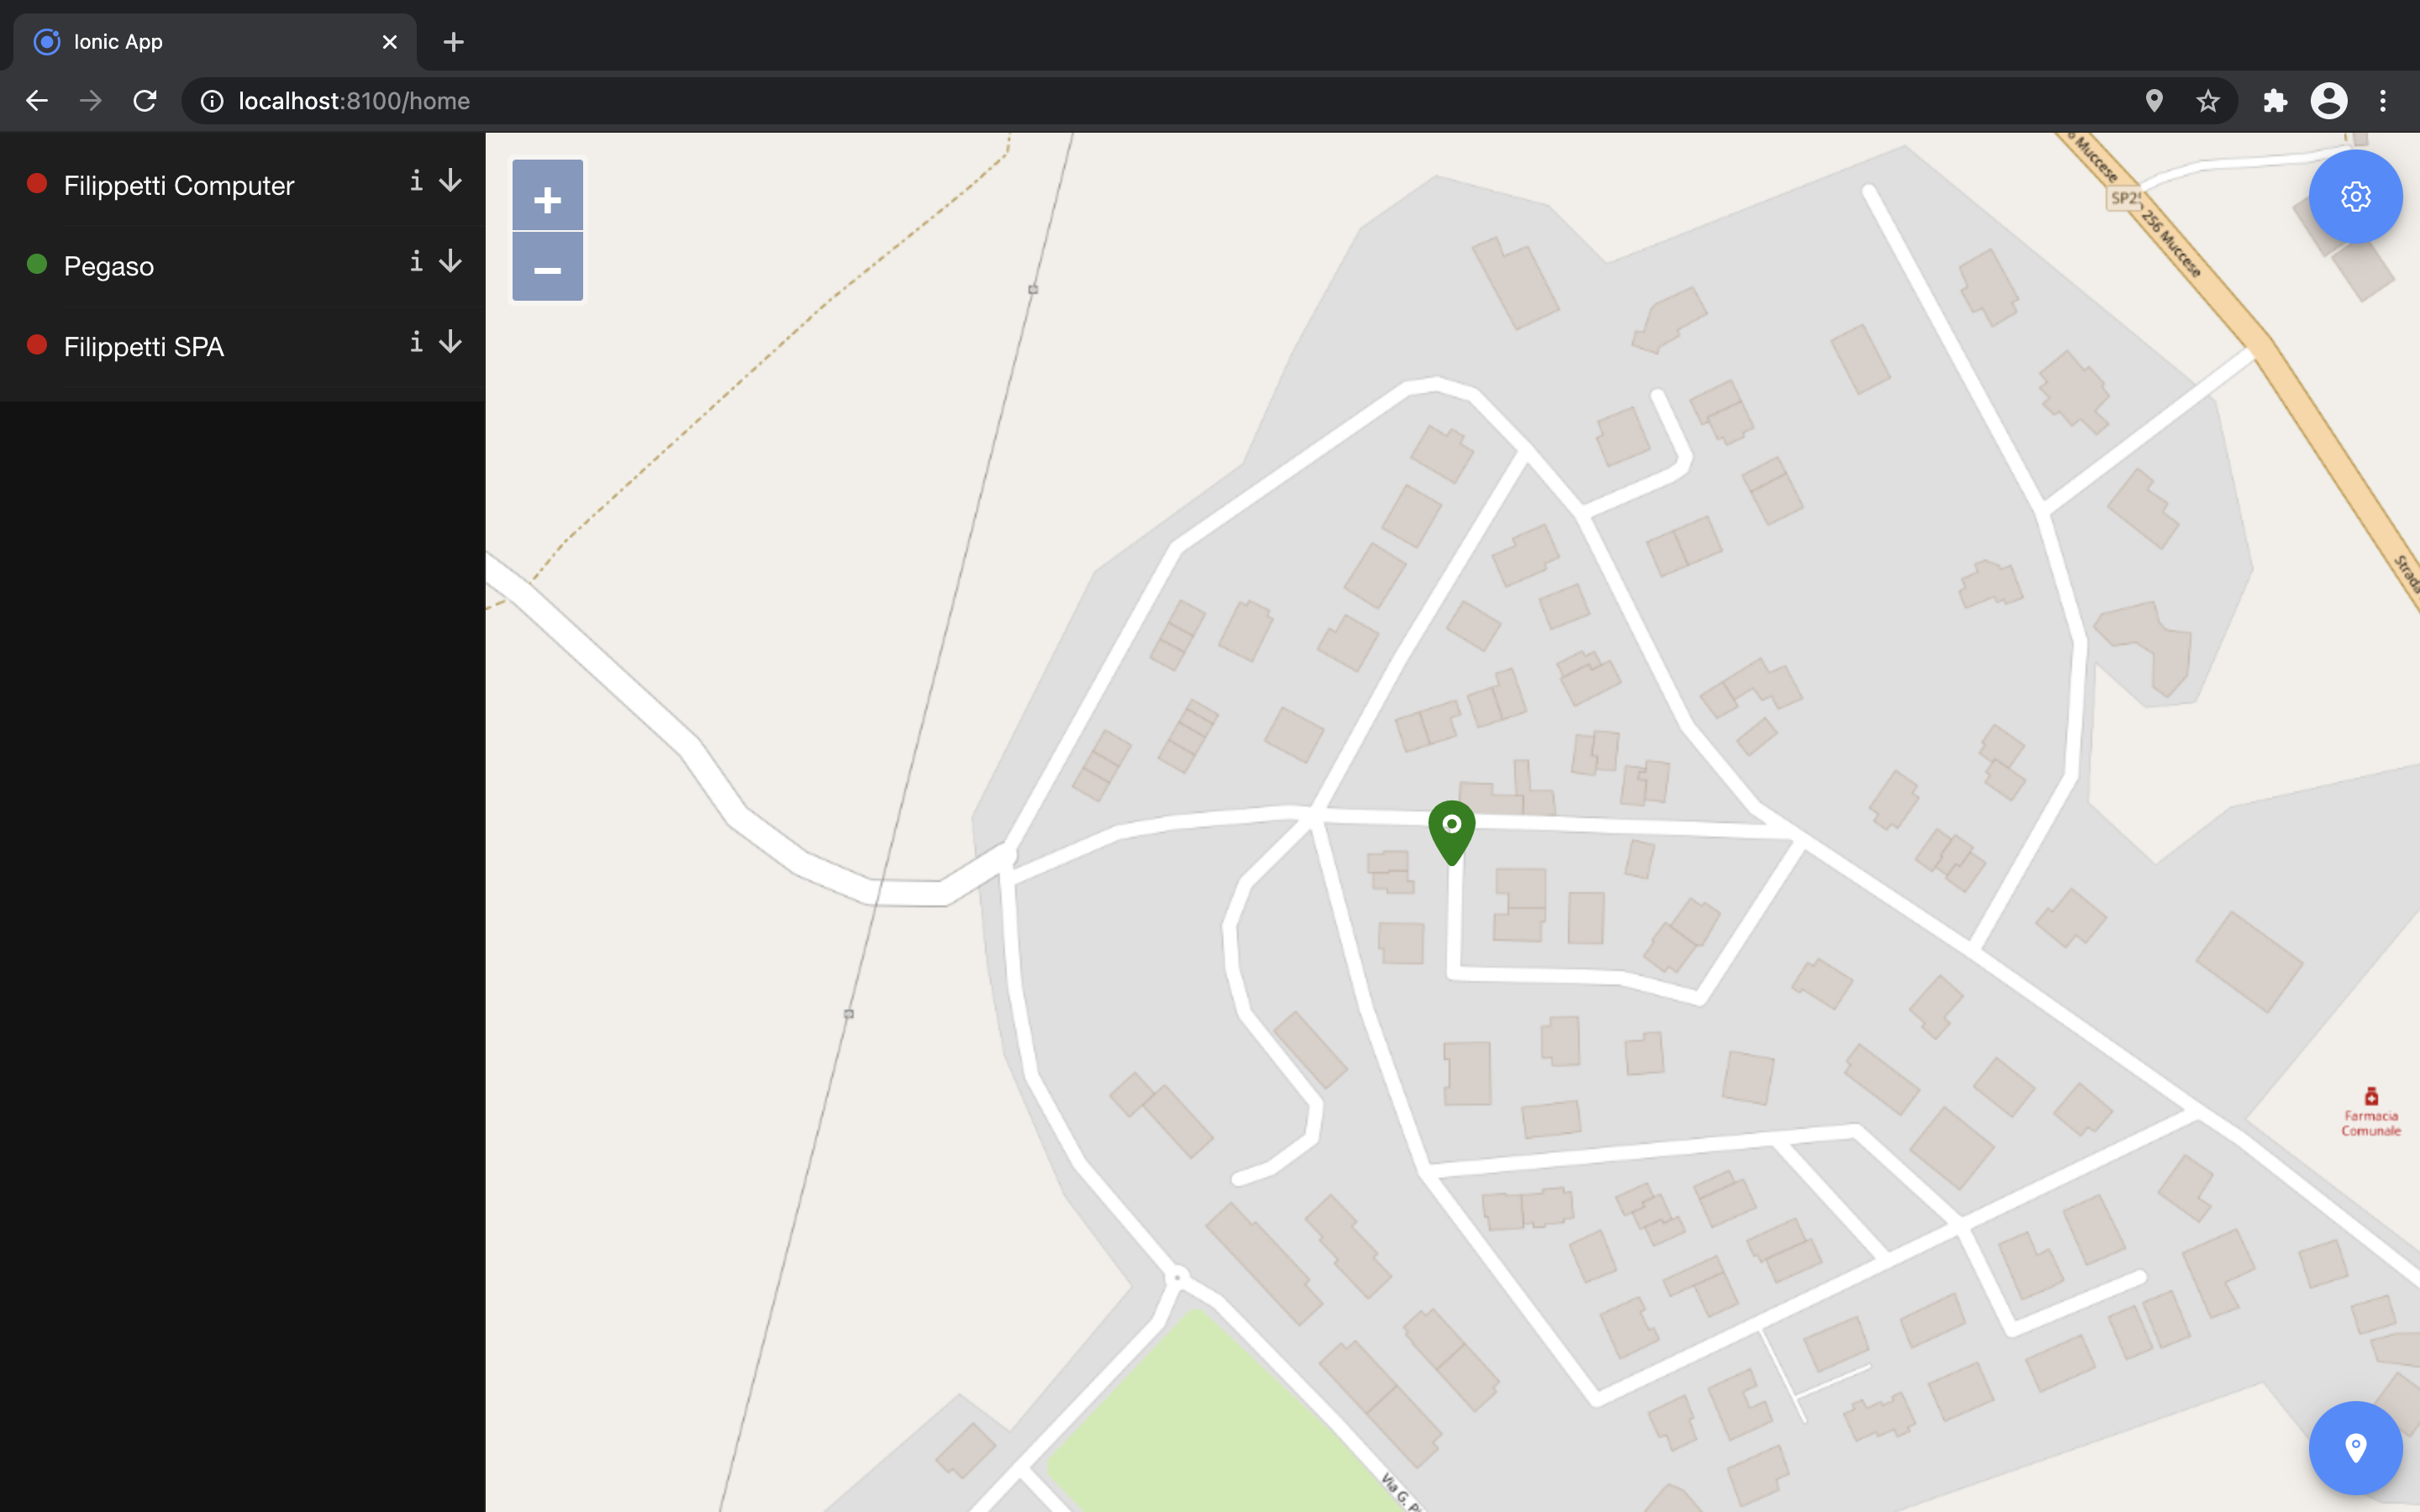
\includegraphics[width=.7\textwidth]{figure/ionicreact_3iterazione_geolocalizzazione.png}\hfill
    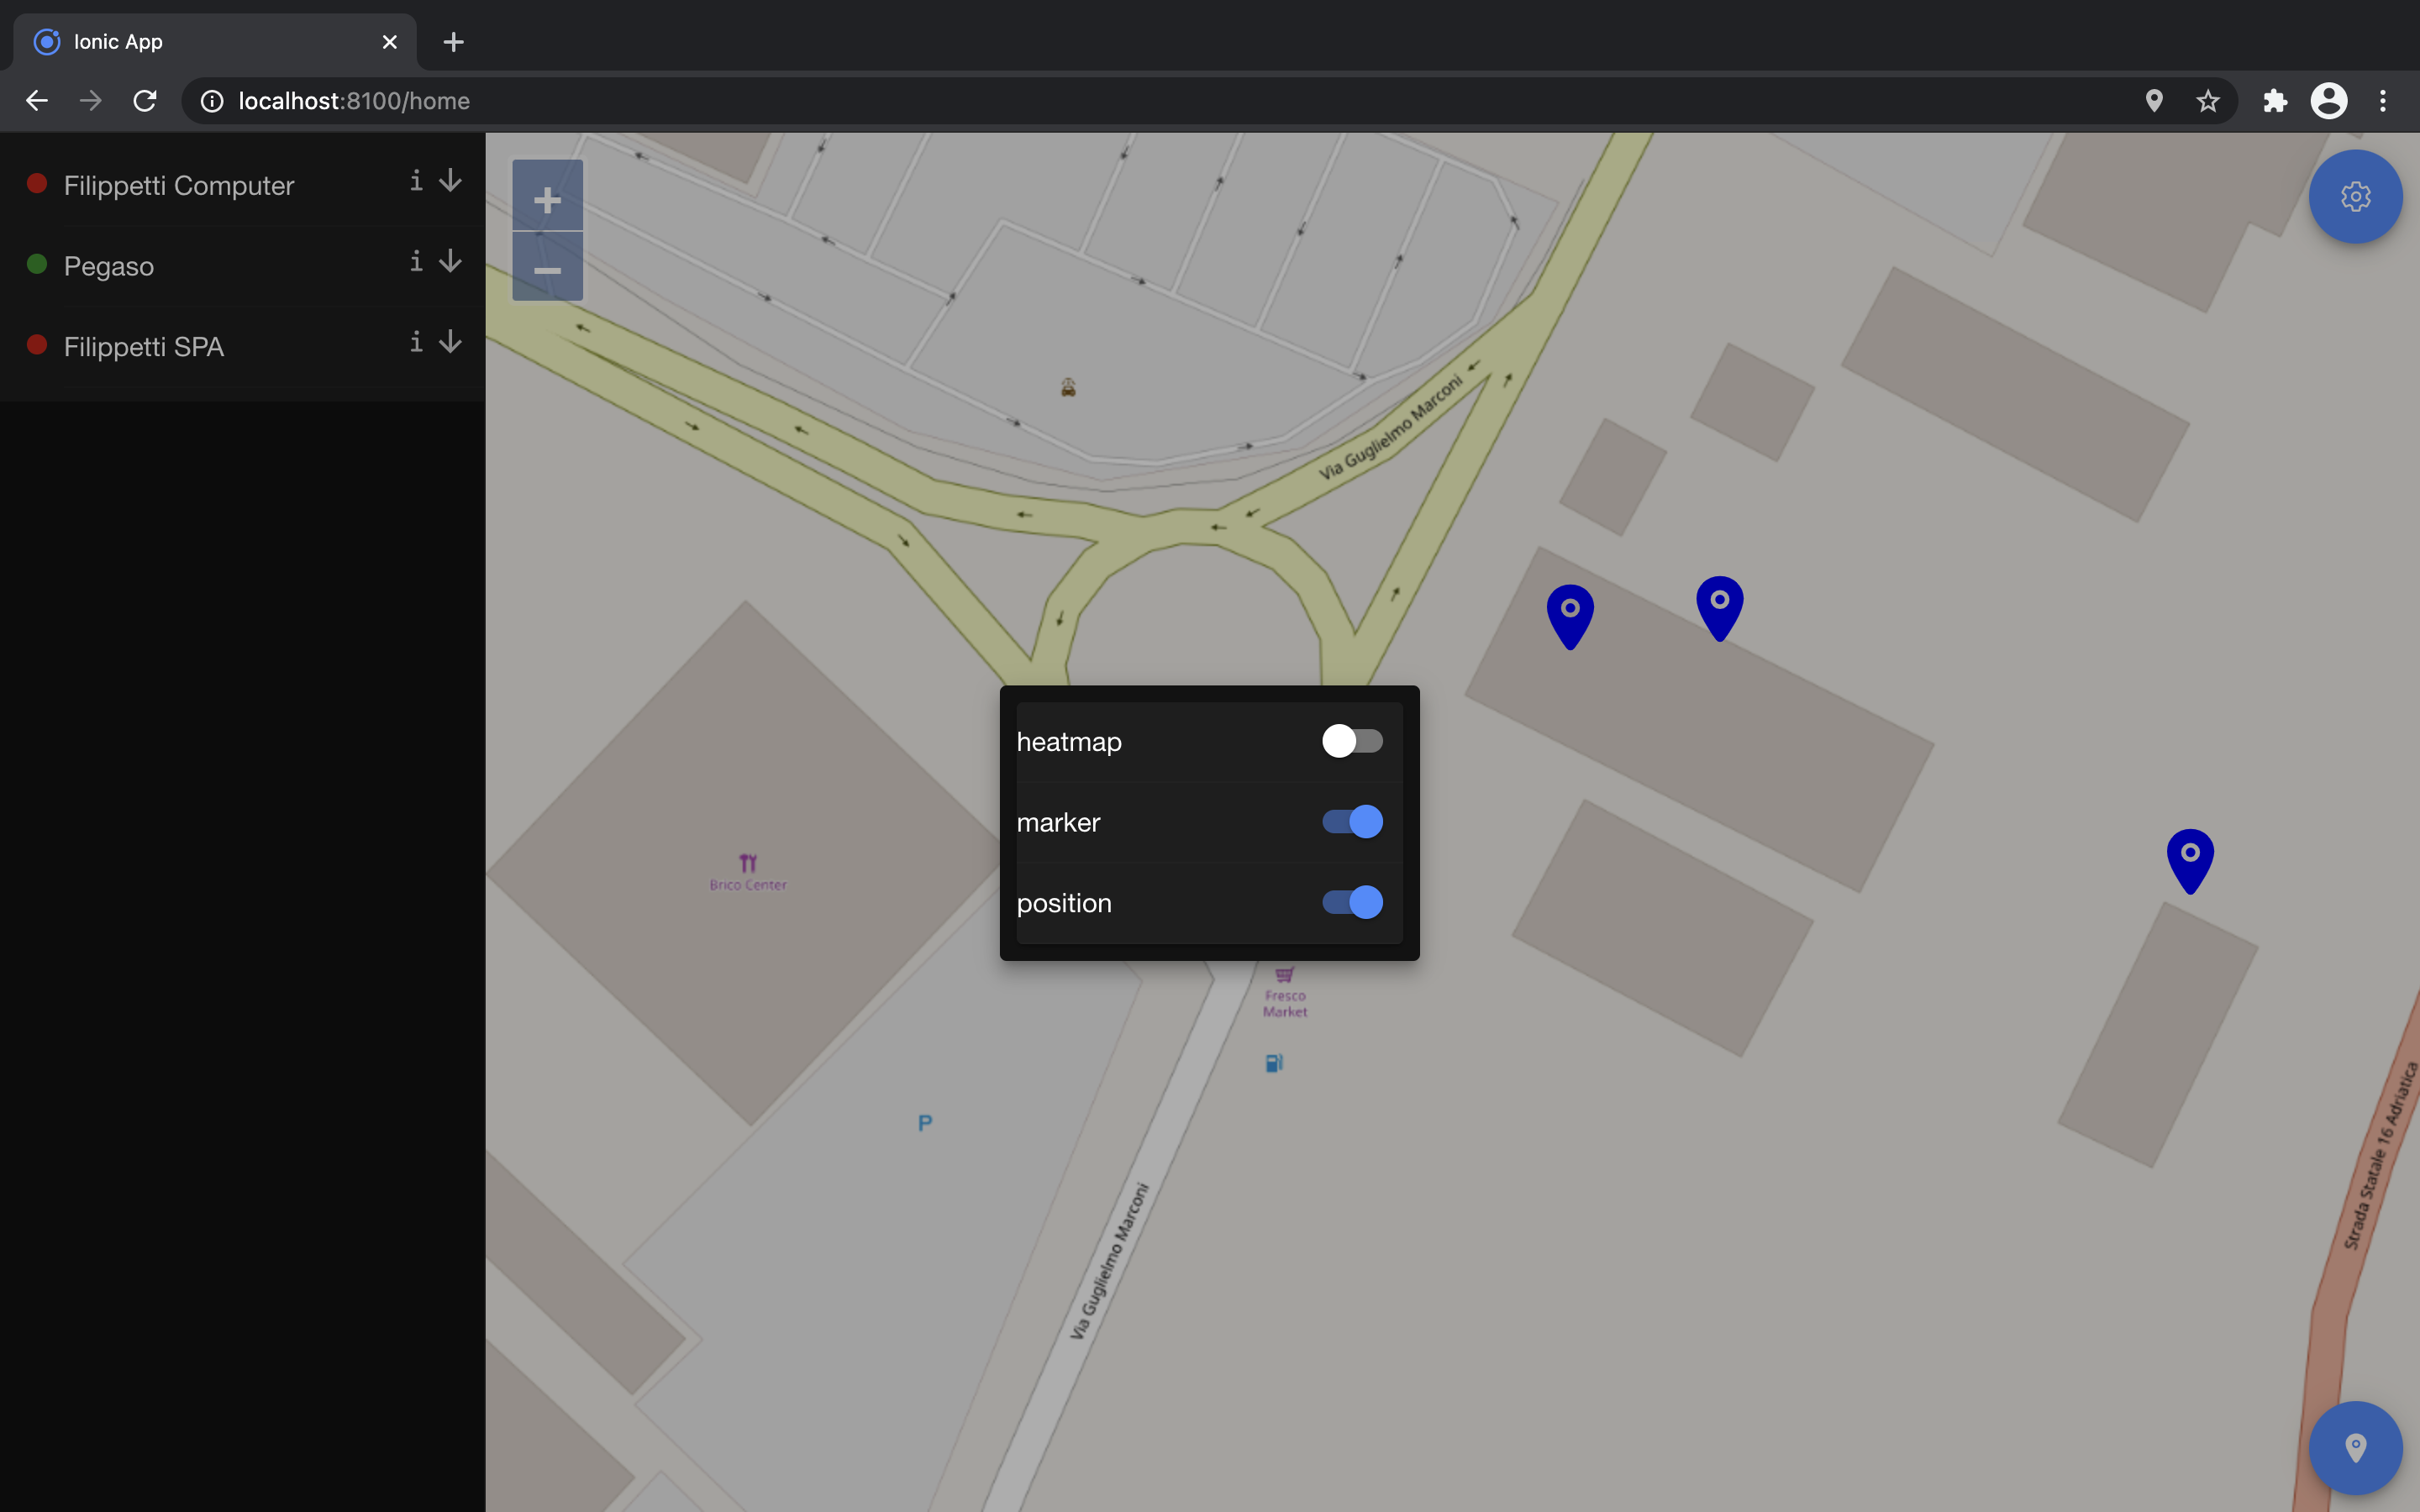
\includegraphics[width=.49\textwidth]{figure/ionicreact_3iterazione_menu1.png}\hfill
    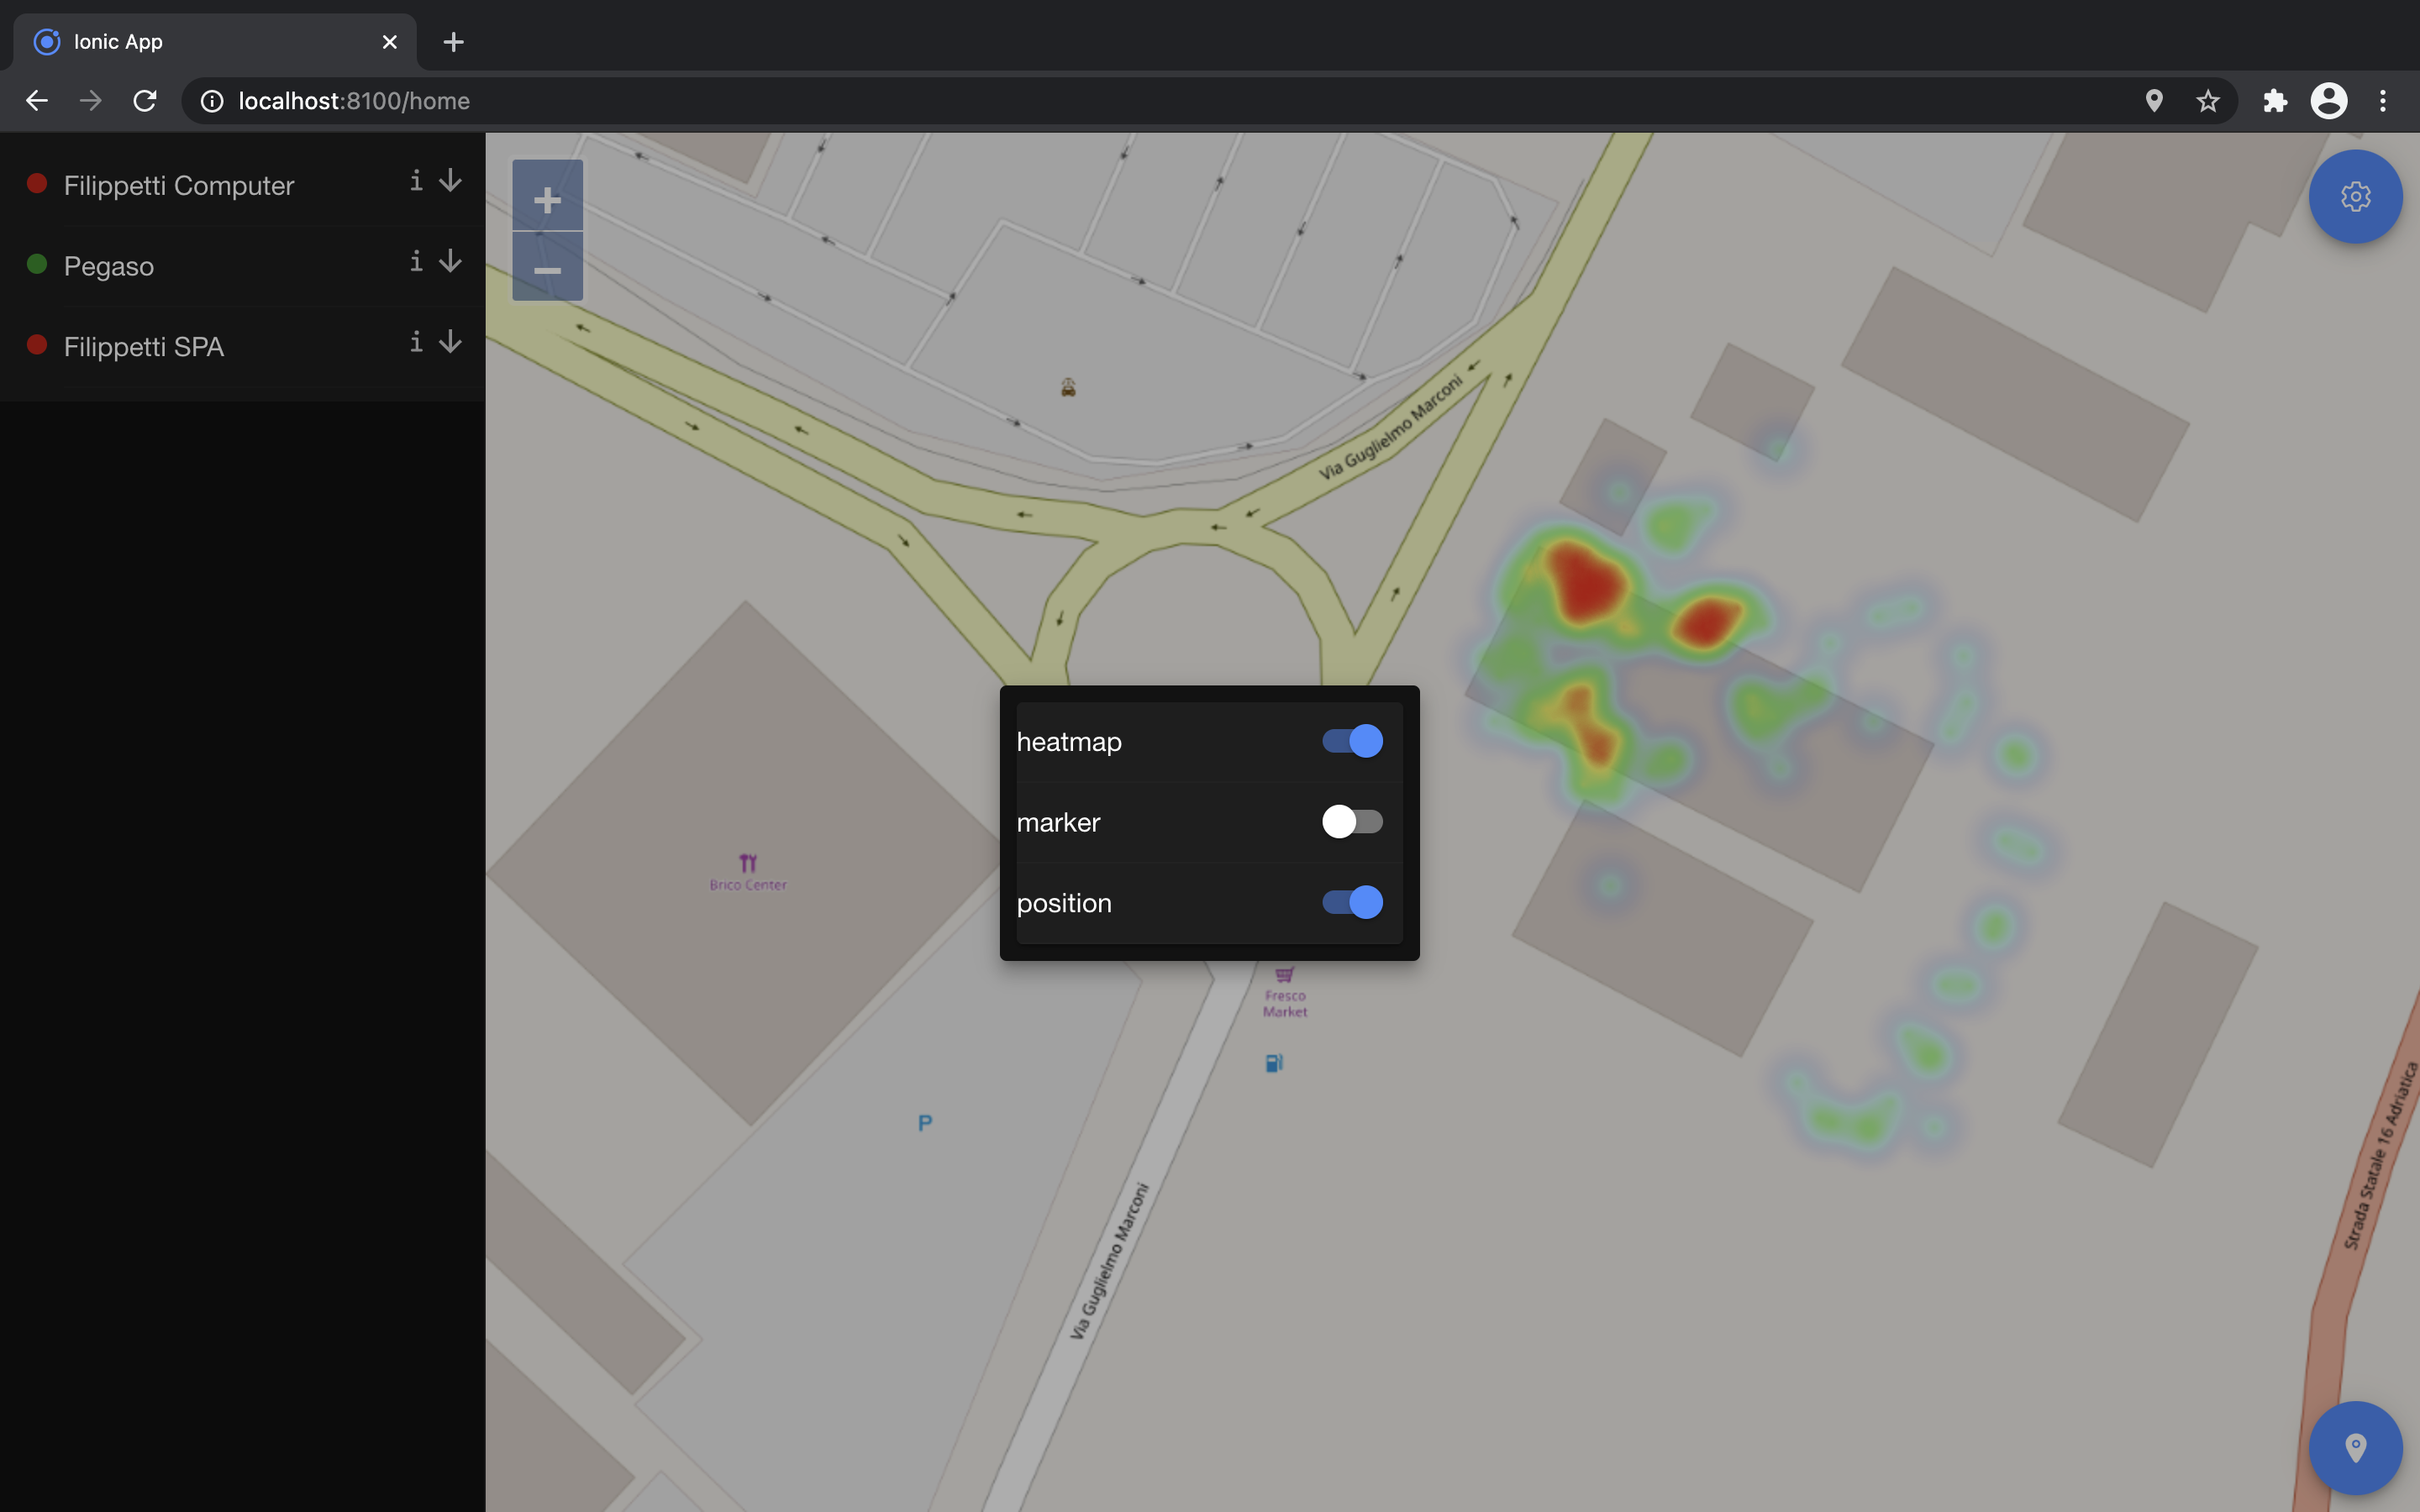
\includegraphics[width=.49\textwidth]{figure/ionicreact_3iterazione_menu2.png}
    \caption{Geolocalizzazione e menu layers}
    \label{IonicReact_3iterazione}
\end{figure}

\addcontentsline{toc}{section}{Riferimenti bibliografici}
\printbibliography

\end{document}